\chapter{Экспериментальные исследования}
\label{cha:chap6}

\section{Алгоритм работы устройства}

Последовательность действий функционирования устройства аналогична с представленной в \ref{cha:chap4}, не считая особенности работы с периферией микроконтроллера, и может быть описана следующим образом:
\begin{enumerate}
	\item <<слепой>> пуск двигателя с фиксированным интервалом смены коммутирующих фаз двигателя;
	\item смена коммутирующих обмоток (выполняется по таймеру, работающему с периодом дискретизации)
	\begin{enumerate}
		\item представление с помощью АЦП выхода датчика тока и напряжений на фазах в численной форме (т. к. у нас одно значение силы тока, то чтобы определить ток по фазам необходимо знать текущее состояние ключей инвертора);
		\item выполнение преобразования Парка для токов и напряжений фаз;
		\item оценка тока и противо-ЭДС по формулам \ref{eq:hat_i} и \ref{eq:hat_e};
		\item фильтрация противо-ЭДС фильтром низких частот первого порядка с частотой среза $f_{\textrm{среза}}$;
		\item оценка положения ротора по формуле \ref{eq:theta_e} и скорости вращения ротора;
		\item оценка электромагнитного момента по формуле \ref{eq:T_e};
		\item получение выхода двухконтурной системы с ПИ регуляторами в диапазоне от $-1$ до $1$, на основе чего определение новой скважности ШИМ и нового состояния ключей инвертора;
		\item смена состояний ключей через драйверы, логика работы которых описана в \ref{sec:inv};
	\end{enumerate}
	\item получение текущего положения ротора по сигналам с компаратора, описанного в \ref{sec:meas_part};
	\item отправка данных с значениями текущей, оценённой скорости и заданной скоростей, силы тока по фазам по протоколу USART (последовательный протокол передачи данных) через DMA (прямое управление памятью).
\end{enumerate}

\section{Результаты эксперимента}

На основе экспериментального стенда, разработанного в \ref{cha:chap5} были проведены экспериментальные исследования.

Параметры, используемые при моделировании:
\begin{enumerate}
	\item параметры ПИ регуляторов контуров скорости и момента, а также параметры двигателя были взяты из \ref{sec:model_res}
	\item параметры наблюдателя:
	\begin{align*}
		&g = 0,95\\
		&\eta = 7,8821e-6\\
		&f_{\textrm{среза}}=30\textrm{ Гц}
	\end{align*}
	\item период дискретизации:
	\begin{align*}
		T_s = 1e-4\textrm{ с}
	\end{align*}
	\item параметры передачи через UART данных:
	\begin{align*}
		&\textrm{Скорость передачи} = 40000 \textrm{ бит/с}\\
		&\textrm{Длина пакета} = 40 \textrm{ бит}
	\end{align*}
\end{enumerate}

Результаты работы стенда приведены на Рисунке \ref{pic:exp_res}. Получилось, что из-за шумов и погрешности в измерении тока и напряжений действительное значение скорости не сходится полностью к заданному, а остаётся в некотором небольшом диапазоне, который, однако, соответствует $1$ \% зоне, определённой в техническом задании. Также перерегулирование и время переходного процесса соответствует желаемым показателям.

\begin{figure}[!h]
\centering
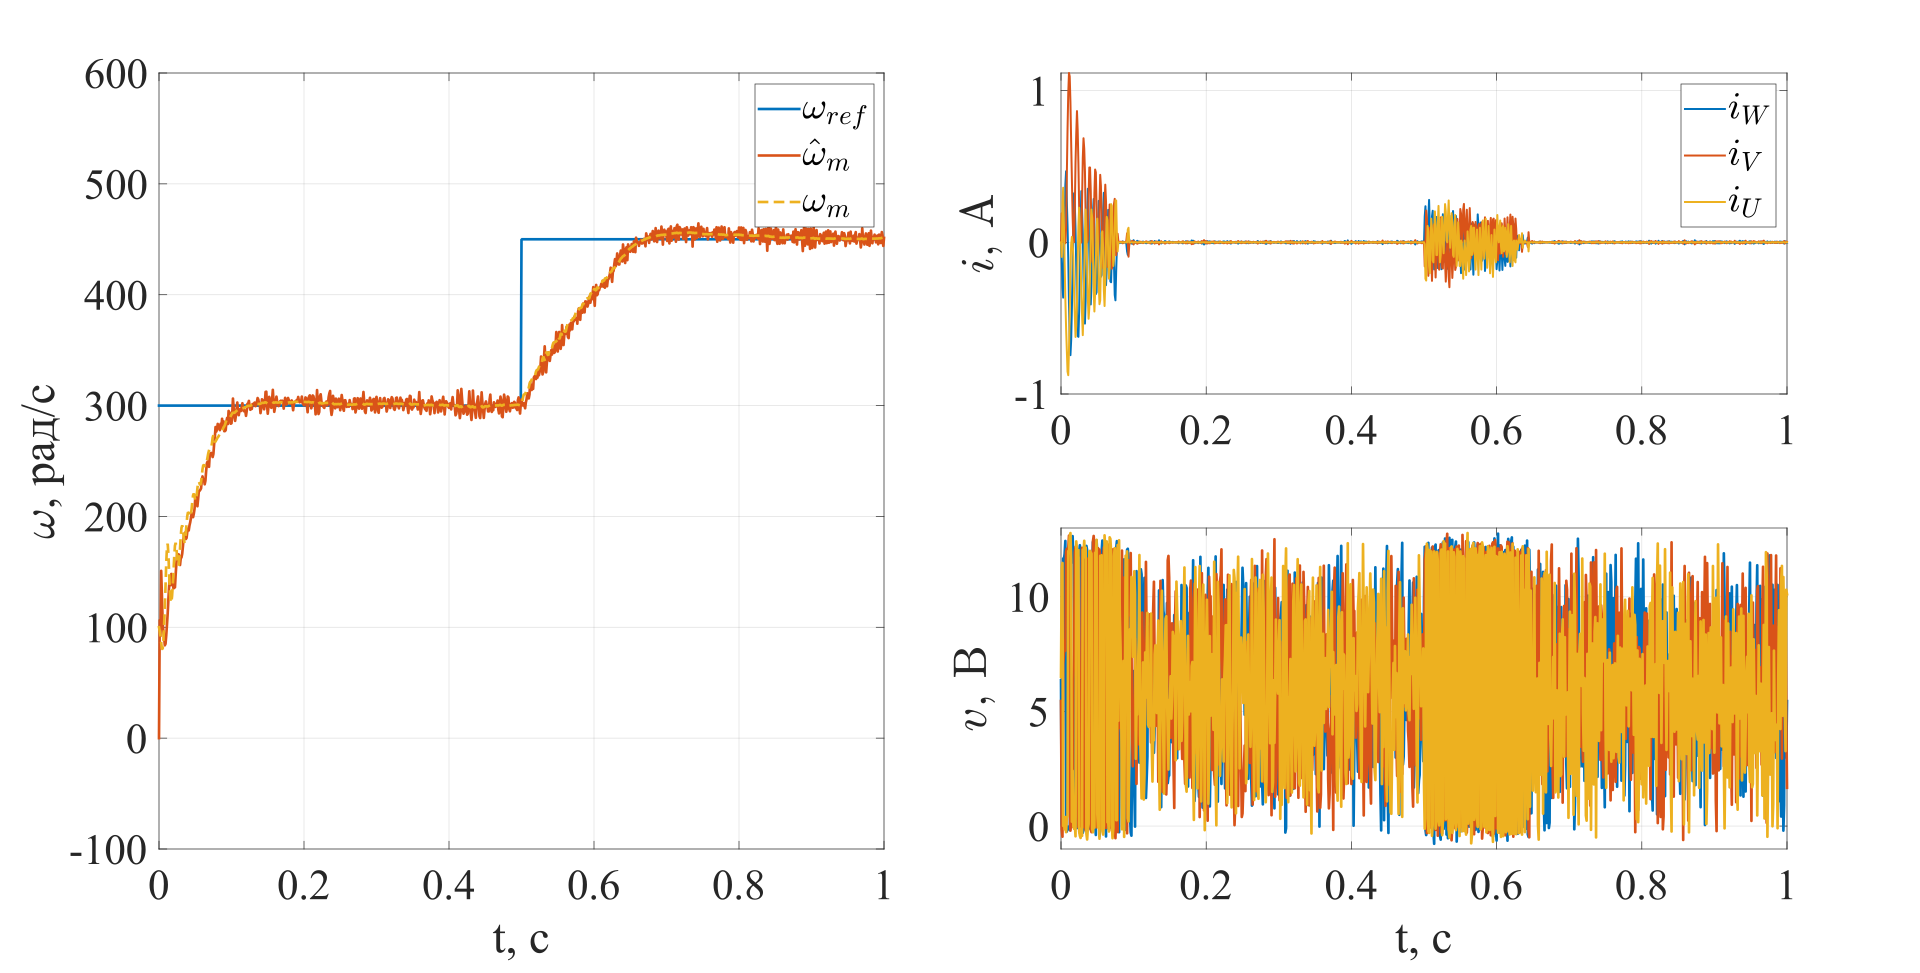
\includegraphics[width=\textwidth]{inc/svg/exp_res}
\caption{результаты эксперимента (слева --- заданная, оцененная и действительная скорость ротора, справа сверху --- токи по фазам, справа снизу --- напряжения по фазам)}
\label{pic:exp_res}
\end{figure}